\chapter{Literature Review}

\section{Preliminaries}

\textbf{Fraud detection as a learning problem.} Transaction fraud detection is a binary classification task on a continuous stream of transactions. Frauds are rare, typically well under 5\% of transactions, so the task is highly imbalanced and accuracy is a misleading measure \cite{abdelnaby2023,aldaoud2025}. Precision and recall of the fraud class, and summary measures such as PR-AUC, describe performance more faithfully. In an operational FDS, investigators can only check a limited number of alerts per day, so the precision of the top-ranked alerts matters most \cite{dalpozzolo2018}.

\textbf{Concept drift.} Model drift is the loss of performance that follows when deployed data no longer resembles the training data \cite{pulicharla2019}. It takes several forms: \textit{concept drift}, where the relationship between features and labels changes; \textit{covariate shift}, where the distribution of the input features changes; and \textit{label drift}, where the frequency of the classes changes \cite{pulicharla2019,kodakandla2024}. Only a change in the relationship between features and labels necessarily harms a model; a change in the inputs may or may not. Drift can also be described by how it unfolds, as illustrated in Figure \ref{fig:drift}. In \textit{sudden} drift the old pattern is replaced at once; in \textit{gradual} drift the old and new patterns alternate, with the new one becoming more frequent; in \textit{incremental} drift the pattern moves slowly through intermediate states; and in \textit{recurring} drift earlier patterns return, for example with seasonal spending. Fraud is an adversarial setting, so drift is frequent, irregular and partly caused by the detection system itself \cite{menezes2025,hassan2026}.

\begin{figure}[htbp]
  \centering
  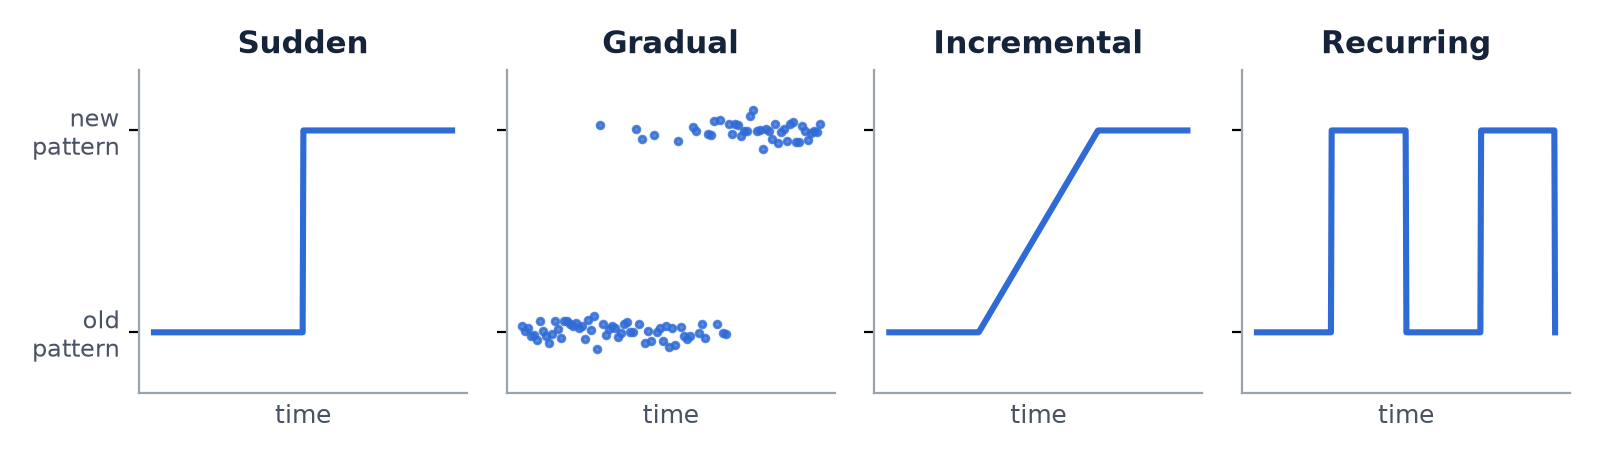
\includegraphics[width=\textwidth]{figures/drift_types.png}
  \caption{Types of concept drift by how the underlying fraud pattern changes over time}
  \label{fig:drift}
\end{figure}

\textbf{Drift detection.} Drift detectors fall into two broad groups. Label-free detectors compare the distribution of recent inputs or model scores with a reference, using measures such as the PSI, the KS test or the Kullback-Leibler divergence \cite{shakil2025,wong2025}; they can run immediately but only see changes in the inputs or the scores. The PSI is commonly read as stable below 0.1, moderately shifted between 0.1 and 0.25, and strongly shifted above 0.25, and Wong and Perumal used 0.25 as their retraining threshold \cite{wong2025}. Error-based detectors such as DDM, EDDM and ADWIN monitor the model's error rate and signal drift when it rises \cite{yelleti2025,aldaoud2025}; they detect real drift but need labels, which in fraud detection arrive late.

\textbf{Verification latency.} In a real FDS, most transactions are labelled only after a delay, when a fraud is reported or when the dispute period ends. A small number of alerted transactions receive quick feedback from investigators. Dal Pozzolo et al. formalised this as verification latency and the alert-feedback interaction, and showed that it changes which data a model can learn from and when \cite{dalpozzolo2018}. Figure \ref{fig:delay} shows the consequence for an automated system. At any moment, the most recent weeks of transactions have already been scored but not yet labelled. Performance can therefore only be measured on older, matured transactions, and a retrained model can only learn from data that ends one label delay before the present. The longer the delay, the later a performance drop is noticed and the older the data a new model is trained on.

\begin{figure}[htbp]
  \centering
  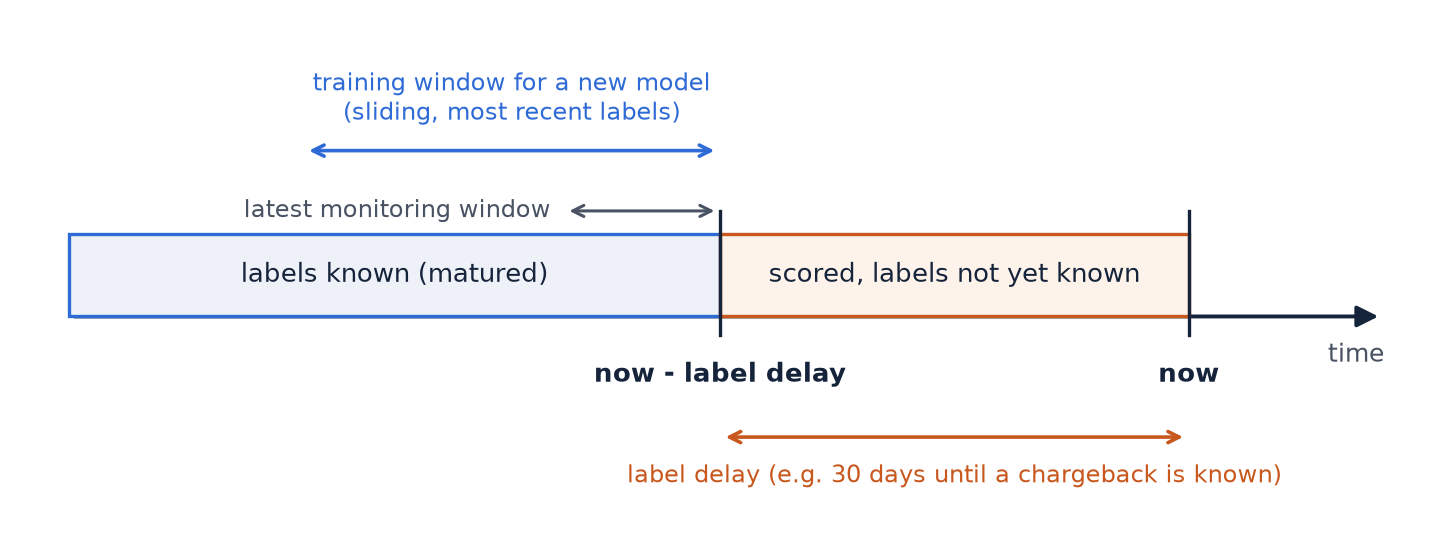
\includegraphics[width=\textwidth]{figures/label_delay.png}
  \caption{Label delay in a fraud detection system: transactions are scored immediately, but their labels become usable only after the delay, which limits both monitoring and retraining}
  \label{fig:delay}
\end{figure}

\textbf{Adaptation strategies.} A deployed model can be kept up to date in several ways. \textit{Periodic} or scheduled retraining rebuilds the model at fixed intervals, while \textit{event-driven} or triggered retraining rebuilds it when a monitoring signal crosses a threshold \cite{pulicharla2019}. The training data may be all history (an expanding window) or only recent data (a sliding window), which forgets outdated patterns \cite{dalpozzolo2018}. \textit{Incremental} or online learning updates the model with every new labelled transaction, and \textit{ensemble} methods combine models trained on different periods \cite{somasundaram2019,yelleti2025}. Which of these works best depends on how quickly labels arrive: under label delay, batch learning can match or beat instance-incremental learning \cite{amekoe2024}.

\textbf{MLOps.} MLOps applies software-engineering practice to the machine-learning lifecycle: automated training pipelines, experiment tracking, versioned model registries, continuous integration and delivery, and monitoring in production \cite{pulicharla2019,kodakandla2024}. Tools such as MLflow, Kubeflow and Apache Airflow automate retraining, while Prometheus, Grafana and Evidently AI support monitoring \cite{pulicharla2019}. Recent MLOps frameworks close the loop between monitoring and retraining for specific domains, such as phishing detection \cite{reda2025} and industrial prediction \cite{wong2025}. A common deployment pattern keeps the model in service (the champion) and promotes a newly trained candidate (the challenger) only if it passes an evaluation, which is the idea behind the promotion gate used in this thesis.

\textbf{Explainability under drift.} Financial regulators expect model decisions to be transparent and auditable, so fraud and credit models are increasingly paired with explanation methods such as SHAP \cite{uddin2026,alessi2026}. Drift affects these explanations too: explanations computed against an outdated reference population can become unstable or unfair as the population changes \cite{john2025}.

\textbf{Evaluation over time.} Evaluating a drifting system requires respecting time: models may only be trained on data from before the period they are tested on \cite{menezes2025}. Common designs include a single chronological split, rolling or walk-forward evaluation, and replaying a historical stream. Because consecutive transactions are correlated, uncertainty estimates should resample whole blocks of time rather than individual transactions.

\section{Review of Existing Research}

\textbf{Fraud detection under drift and label delay.} Dal Pozzolo et al. \cite{dalpozzolo2018} provided one of the most realistic models of a credit-card fraud detection system. Working with an industrial partner and more than 75 million e-commerce transactions collected over three years, they described the layers of an FDS, from terminal checks and blocking rules to the data-driven model and human investigators. They formalised verification latency and the alert-feedback interaction, argued that alert precision is the most meaningful performance measure, and proposed training separate classifiers on recent investigator feedback and on delayed labels, then aggregating their outputs. Their experiments showed that giving more weight to recent feedback produced more precise alerts, and that sliding-window and ensemble approaches handled drift. The work is the foundation for treating label delay as a first-class concern. Its limitations for this thesis are that the data is private, that the timing of retraining is not studied, and that the model is not embedded in an MLOps workflow with monitoring and safe deployment.

Amekoe et al. \cite{amekoe2024} compared instance-incremental learning with batch learning for fraud detection when labels arrive with a delay. Instance-incremental algorithms are usually preferred for evolving streams, but they assume that each label is available immediately. Using fraud detection data and generated datasets, the authors found that instance-incremental learning, including the Adaptive Random Forest, was not the superior option compared with batch-trained models such as XGBoost, and that batch solutions are also easier to interpret. This finding directly supports the design choice of this thesis to retrain a batch model on windows of delayed labels. The study compares learning paradigms, however, and does not examine when to retrain or how to deploy a new model safely.

Yelleti \cite{yelleti2025} proposed ROSFD, a two-stage framework for online streaming fraud detection. An initial model is built offline with incremental learning to avoid a cold start, and in production the drift detectors DDM, EDDM and ADWIN decide when the model is retrained incrementally. Across five datasets, ADWIN gave the best results among the detectors and the Adaptive Random Forest achieved the highest AUC on four of them, while the train-only-when-required strategy substantially reduced how often the model was retrained without a large loss of AUC. The study is close to the question of this thesis, since it tests retraining only when needed. It reports ROC-AUC, which is less informative than PR-AUC for rare fraud, and it assumes labels are available immediately, which makes error-based detectors look more responsive than they would be in practice.

Somasundaram and Reddy \cite{somasundaram2019} proposed a parallel and incremental fraud detection model, Transaction Window Bagging, which combines parallel bagging, incremental learning, cost-sensitive learning and weighted voting to handle concept drift and class imbalance together. Evaluated on Brazilian bank data, it improved the fraud detection rate and the misclassification cost compared with other models. The study is valuable because it treats fraud detection as a continuous stream rather than a static dataset. However, the data is private, label delay is not modelled, and the effect of retraining frequency is not isolated.

Al-Daoud and Abu-AlSondos \cite{aldaoud2025} proposed a hybrid machine-learning framework for fraud detection in Gulf Cooperation Council banks that addresses class imbalance (SMOTEBoost and cost-sensitive learning), adversarial attacks (adversarial training and a FraudGAN), concept drift (DDM and ADWIN) and explainability (SHAP, LIME and human-in-the-loop review). On real bank transactions, the framework raised fraud recall from 35\% to 85\%, reduced the success rate of adversarial attacks from 35\% to 5\%, and recovered from drift within 24 hours while keeping latency below 150 milliseconds. The study shows that drift handling must work together with the other demands of a production fraud system. Drift, however, is one component among many, the retraining policy is not compared with alternatives, and the private data prevents replication.

Alessi and Fugini \cite{alessi2026} developed a real-time financial fraud detection system for transaction data streams that addresses extreme class imbalance and concept drift. It uses a lightweight data stream management system for real-time feature engineering, combines deterministic rules with adaptive machine-learning models, manages the decision threshold dynamically to balance precision and recall, and compares several adaptive learning strategies. It also introduces an interpretability framework that turns low-level feature attributions into concepts investigators can act on. The work demonstrates a practical, operational view of adaptive fraud detection, but it does not test safeguards against faulty model updates or evaluate the effect of label delay on the retraining decision.

Menezes and Filho \cite{menezes2025} studied how graph neural network fraud detectors degrade under natural data drift. They built a heterogeneous knowledge graph from 284,000 IEEE-CIS transactions, trained R-GCN, HGT and HAN models on the earliest 70\%, and then froze the models and monitored them over 50 subsequent 12-hour windows. All models degraded in a volatile, non-monotonic way; the F1-score of HGT fell from 0.747 to as low as 0.455, while the simpler R-GCN was the most stable. They also observed that AUC stayed stable while F1 fluctuated, suggesting that score distributions shift and fixed decision thresholds become outdated. The study is directly relevant because it uses the same dataset and confirms that drift is a real problem on it. However, it only measures degradation: no retraining strategy is evaluated, label delay is not modelled, and the proposed mitigation framework is conceptual.

Hassan \cite{hassan2026} proposed DriftGuard-TriAudit, a concept-drift-aware continual learning framework for financial statement fraud that jointly analyses financial ratios, management discussion text and document layout. It adds modality-specific drift monitoring, reliability-weighted fusion of the three modalities, and memory-based continual learning. On a synthetic benchmark with four temporal fraud scenarios, it achieved an average precision of 0.628 and improved precision over standard continual fine-tuning (0.547 against 0.428) with a similar AUC. The work shows that drift-aware continual learning is relevant beyond transaction fraud, but it concerns a different kind of fraud and is evaluated only on synthetic data.

\textbf{Retraining decisions and MLOps.} Shakil et al. \cite{shakil2025} proposed a feature-drift-guided retraining framework for MLOps. They combined the KS statistic with a confidence-based model performance indicator and a new feature-level indicator, the percent mean shift, and retrained a model only when all three signalled drift and enough drifted data was available. Using simulated mean and variance shifts on health, loan-approval and benchmark datasets with Random Forest and SVM models, they showed that the percent mean shift correlated with performance loss more strongly than the KS statistic alone, and that the framework matched existing drift detectors while retraining less often. The study addresses exactly the question of when retraining is warranted. Its drift is artificially induced into one feature at a time, however, the datasets are not fraud streams, label delay is ignored, and the confidence-based indicator does not measure whether predictions are correct.

Wong and Perumal \cite{wong2025} proposed an AI-driven model-retraining architecture that combines drift detection (the KS test and ADWIN, with PSI and Kullback-Leibler divergence to measure severity), an agentic orchestrator that schedules retraining using a reinforcement-learning policy, and data-governance controls with a composite data-quality index. In a smart-manufacturing case study with injected sensor drift, the architecture raised the F1-score from 0.62 after drift to 0.93, and outperformed a weekly retraining schedule while retraining only three times in six months. Its strengths are the integration of retraining with data quality and the explicit comparison with scheduled retraining. The evidence is, however, limited to one dataset with artificially controlled drift, reported without confidence intervals or repeated runs, and labels are assumed to be available immediately. The comparison with scheduled retraining is therefore an important claim that this thesis re-examines on real fraud data with label delay.

Reda et al. \cite{reda2025} presented HAMF, a hybrid MLOps framework that manages the whole lifecycle of adaptive phishing detection models. Its microservices architecture links data ingestion, SHAP-guided feature replacement, event-driven retraining, monitoring, fairness auditing and stakeholder feedback in a closed loop of 13 pipeline stages. On three phishing datasets, it detected drift within 18 seconds, recovered an F1-score above 0.99 after drift, reduced fairness disparity by 60\%, and handled 2,300 requests per second with a p99 latency below 50 milliseconds, outperforming SageMaker and Kubeflow with MLflow baselines. HAMF is a strong example of a complete, closed-loop MLOps framework. Phishing detection, however, receives labels far faster than card fraud, so its event-driven design cannot be transferred directly to a setting with weeks of label delay.

Kodakandla \cite{kodakandla2024} described an end-to-end MLOps approach for detecting and mitigating data drift in real-time systems across healthcare, finance and the Internet of Things, combining automated drift detection, retraining techniques and adaptive models with attention to governance and ethics. Pulicharla \cite{pulicharla2019} reviewed methods for detecting model drift and automating retraining in ML pipelines, covering statistical tests, drift detection algorithms, monitoring tools and retraining pipelines, and discussed the trade-off between scheduled and event-driven retraining. These works describe what an MLOps system for drifting data should contain, but they are conceptual and do not measure which retraining policy works best for fraud detection under label delay.

Kaushik et al. \cite{kaushik2025} proposed an architecture for real-time analytics that embeds machine-learning detection into streaming data pipelines built on Kafka and Flink. It includes a feedback-driven module for online model updates, adaptive stream operators, hybrid edge-cloud execution and a self-healing pipeline. In simulation, an adaptive random forest with feedback achieved higher detection accuracy and a lower false-positive rate than static Isolation Forest and k-NN detectors, with lower latency. The paper usefully places fraud detection within a production data architecture. Its evaluation is based on simulated workloads and synthetic data, so its results cannot show how such a system behaves on real fraud streams or under label delay.

\textbf{Explainability under drift.} Uddin and Aziz \cite{uddin2026} proposed a SHAP-guided adaptive ensemble for explainable financial fraud detection and checked it against U.S. regulatory requirements. Using the 590,540 transactions of IEEE-CIS, they found that XGBoost with TreeExplainer gave nearly perfectly stable explanations, while an LSTM's explanations were weak; the adaptive ensemble reached an AUC-ROC of 0.8837 on held-out data, and a GraphSAGE model reached 0.9248. John \cite{john2025} studied credit scoring under concept drift and showed that SHAP explanations computed against a fixed background become unstable and unfair as populations change; drift-aware rebaselining of the background and online surrogate calibration improved stability and reduced disparate impact without hurting accuracy. Together, these studies indicate that a model's explanations, not only its predictions, need maintenance under drift, which is a natural extension of the framework in this thesis.

\textbf{Static fraud classification.} A large group of studies focuses on maximising performance on a static dataset. Mienye and Sun \cite{mienye2023} proposed a deep-learning ensemble with LSTM and GRU base learners, a multilayer perceptron meta-learner and SMOTE-ENN resampling, and reported a sensitivity of 1.000 and a specificity of 0.997. Sohony et al. \cite{sohony2018} combined feed-forward neural networks and random forests in an ensemble to balance fraud recall against false alarms. Abd El-Naby et al. \cite{abdelnaby2023} combined balancing methods such as SMOTE, Borderline-SMOTE, ADASYN and SMOTETomek with classical classifiers and reported high accuracy after balancing. Dang et al. \cite{dang2021} compared resampling methods, classical models and deep reinforcement learning, and showed that resampling before the train-test split can make results look far better than they are. These studies establish strong classifiers and careful imbalance handling, but they use random splits of static data, so they do not show how the models would perform after deployment.

Table \ref{tab:review} summarises the studies most closely related to this thesis.

{\footnotesize
\begin{longtable}{>{\raggedright\arraybackslash}p{0.16\textwidth}>{\raggedright\arraybackslash}p{0.19\textwidth}>{\raggedright\arraybackslash}p{0.19\textwidth}>{\raggedright\arraybackslash}p{0.11\textwidth}>{\raggedright\arraybackslash}p{0.29\textwidth}}
\caption{Summary of the most closely related studies}\label{tab:review}\\
\toprule
\textbf{Study} & \textbf{Data} & \textbf{Drift handling} & \textbf{Label delay} & \textbf{Main limitation for this thesis} \\
\midrule
\endfirsthead
\toprule
\textbf{Study} & \textbf{Data} & \textbf{Drift handling} & \textbf{Label delay} & \textbf{Main limitation for this thesis} \\
\midrule
\endhead
Dal Pozzolo et al. \cite{dalpozzolo2018} & 75M+ real card transactions, 3 years & Sliding window and ensembles; separate feedback and delayed models & Yes (core) & Private data; retraining timing and MLOps integration not studied \\ \midrule
Amekoe et al. \cite{amekoe2024} & Fraud data and generated streams & Instance-incremental vs. batch learning & Yes (core) & No drift-triggered retraining or safe deployment \\ \midrule
Yelleti \cite{yelleti2025} & Five fraud datasets & DDM, EDDM, ADWIN trigger incremental retraining & No & Evaluated with ROC-AUC only; labels assumed immediate \\ \midrule
Al-Daoud and Abu-AlSondos \cite{aldaoud2025} & Private GCC bank transactions & DDM and ADWIN with adaptive learning & No & Private data; drift handled as one part of a larger framework \\ \midrule
Alessi and Fugini \cite{alessi2026} & Transaction data streams & Compares adaptive learning strategies; dynamic threshold & Not central & No promotion checks or fault testing \\ \midrule
Somasundaram and Reddy \cite{somasundaram2019} & Brazilian bank data & Transaction-window bagging, incremental & No & Private data; no label delay \\ \midrule
Menezes and Filho \cite{menezes2025} & IEEE-CIS (subset) as a graph & None: frozen models monitored & No & Measures decay only; no retraining evaluated \\ \midrule
Shakil et al. \cite{shakil2025} & Health, loan and benchmark datasets & KS + mean-shift indicator triggers retraining & No & Artificially induced drift; not fraud \\ \midrule
Wong and Perumal \cite{wong2025} & Manufacturing sensor data & PSI/KL + ADWIN, agentic retraining scheduler & No & Injected drift; single run; no confidence intervals \\ \midrule
Reda et al. \cite{reda2025} & Phishing URL datasets & Event-driven retraining in a closed-loop MLOps pipeline & No & Different domain; drift simulated \\ \midrule
Mienye and Sun \cite{mienye2023} & Public card datasets & None (static) & No & Random split with resampling; no temporal evaluation \\ \bottomrule
\end{longtable}
}

\section{Summary of Key Findings}

The literature agrees that concept drift is a real and serious problem for fraud detection. Static models degrade after deployment, sometimes sharply and irregularly \cite{menezes2025,dalpozzolo2018}, and fraud detection systems therefore need a way to update their models over time. Sliding windows, incremental learning, ensembles and drift-triggered retraining have all been proposed \cite{dalpozzolo2018,somasundaram2019,yelleti2025,aldaoud2025,alessi2026}.

Label delay is a defining feature of fraud detection but is rarely modelled. Dal Pozzolo et al. and Amekoe et al. showed its importance \cite{dalpozzolo2018,amekoe2024}, yet most retraining frameworks assume that labels are immediately available \cite{shakil2025,wong2025,yelleti2025,kaushik2025}. Because error-based drift detectors depend on labels, label delay directly limits how quickly any performance-based trigger can react.

Recent MLOps research favours retraining triggered by drift detection, and reports that it outperforms or matches scheduled retraining with fewer retrains \cite{shakil2025,wong2025,yelleti2025}. These claims rest on artificially induced drift, single datasets, non-fraud domains or immediate labels. At the same time, statistical drift does not always correspond to a loss of performance \cite{shakil2025}. Whether drift-triggered retraining is better for fraud detection under realistic conditions is therefore unresolved.

Evaluation practice is a further gap. Many fraud studies report very high results from random splits of static data \cite{mienye2023,abdelnaby2023}, which says little about performance after deployment. Few studies use time-ordered evaluation, confidence intervals, fair tuning of competing strategies or repeated runs, and studies with realistic streams often use private data that cannot be reproduced \cite{dalpozzolo2018,somasundaram2019,aldaoud2025}.

Safe deployment of retrained models also receives little attention. MLOps frameworks close the loop between monitoring and retraining \cite{reda2025,kodakandla2024}, and some compare a new model with the current one \cite{wong2025}, but we found no fraud detection study that tests whether such safeguards actually stop models trained on corrupted labels or features. Finally, drift also affects the stability of explanations \cite{john2025,uddin2026}, which matters for regulated financial systems.

Based on these findings, this thesis proposes a drift-aware continuous learning MLOps framework for financial transaction fraud detection that: (1) is evaluated on public data in strict time order, with confidence intervals, walk-forward tuning and repeated seeds; (2) models label delay explicitly and measures how it limits the benefit of retraining; (3) compares scheduled and drift-triggered retraining fairly and retrains only when the evidence shows it is necessary; (4) monitors performance on delayed labels rather than relying only on label-free drift signals; (5) protects production with a promotion gate and a performance safety net, tested by fault injection; and (6) is released as reproducible open-source code with a second dataset for replication. The following chapters describe the requirements, the methodology and the results of this framework in detail.
